\begin{comment}
\documentclass[10pt]{article}
\usepackage{fullpage, graphicx, url}
\setlength{\parskip}{1ex}
\setlength{\parindent}{0ex}
\title{madsr}
\begin{document}


\begin{tabular}{ccc}
The Alternative Csound Reference Manual & & \\
Previous & &Next

\end{tabular}

%\hline 
\end{comment}
\section{madsr}
madsr�--� Calculates the classical ADSR envelope using the linsegr mechanism. \subsection*{Description}


  Calculates the classical ADSR envelope using the linsegr mechanism. 
\subsection*{Syntax}


 ar \textbf{madsr}
 iatt, idec, islev, irel [, idel] [, ireltim]


 kr \textbf{madsr}
 iatt, idec, islev, irel [, idel] [, ireltim]
\subsection*{Initialization}


 \emph{iatt}
 -- duration of attack phase 


 \emph{idec}
 -- duration of decay 


 \emph{islev}
 -- level for sustain phase 


 \emph{irel}
 -- duration of release phase. 


 \emph{idel}
 -- period of zero before the envelope starts 


 \emph{ireltim}
 (optional, default=-1) -- Control release time after receiving a MIDI noteoff event. If less than zero, the longest release time given in the current instrument is used. If zero or more, the given value will be used for release time. Its default value is -1. (New in Csound 3.59 - not yet properly tested) 


  Please note that the release time cannot be longer than 32767/\emph{kr}
 seconds. 
\subsection*{Performance}


  The envelope is the range 0 to 1 and may need to be scaled further. The envelope may be described as: 


 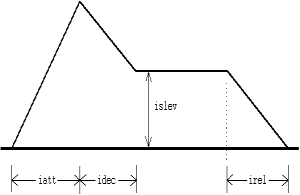
\includegraphics[scale=1]{adsr} 


 Picture of an ADSR envelope.


  The length of the sustain is calculated from the length of the note. This means \emph{adsr}
 is not suitable for use with MIDI events. The opcode \emph{madsr}
 uses the \emph{linsegr}
 mechanism, and so can be used in MIDI applications. 
\subsection*{Examples}


  Here is an example of the madsr opcode. It uses the files \emph{madsr.orc}
 and \emph{madsr.sco}
. 


 \textbf{Example 1. Example of the madsr opcode.}

\begin{lstlisting}
/* madsr.orc */
/* Written by Iain McCurdy */
; Initialize the global variables.
sr = 44100
kr = 441
ksmps = 100
nchnls = 1

; Instrument #1.
instr 1
  ; Attack time.
  iattack = 0.5
  ; Decay time.
  idecay = 0
  ; Sustain level.
  isustain = 1
  ; Release time.
  irelease = 0.5
  aenv madsr iattack, idecay, isustain, irelease

  a1 oscili 10000, 440, 1
  out a1*aenv
endin
/* madsr.orc */
        
\end{lstlisting}
\begin{lstlisting}
/* madsr.sco */
/* Written by Iain McCurdy */
; Table #1, a sine wave.
f 1 0 1024 10 1

; Leave the score running for 6 seconds.
f 0 6

; Play Instrument #1 for two seconds.
i 1 0 2
e
/* madsr.sco */
        
\end{lstlisting}
\subsection*{See Also}


 \emph{adsr}
, \emph{mxadsr}
, \emph{xadsr}

\subsection*{Credits}


 November 2002. Thanks to Rasmus Ekman, added documentation for the \emph{ireltim}
 parameter.


 December 2002. Thanks to Iain McCurdy, added an example.


 December 2002. Thanks to Istvan Varga, added documentation about the maximum release time.


 New in Csound version 3.49.
%\hline 


\begin{comment}
\begin{tabular}{lcr}
Previous &Home &Next \\
maca &Up &mandol

\end{tabular}


\end{document}
\end{comment}
